%%%%%%%%%%%%%%%%%%%%%%%%%%%%%%%%%%%%%%%%%
% Short Sectioned Assignment
% LaTeX Template
% Version 1.0 (5/5/12)
%
% This template has been downloaded from:
% http://www.LaTeXTemplates.com
%
% Original author:
% Frits Wenneker (http://www.howtotex.com)
%
% License:
% CC BY-NC-SA 3.0 (http://creativecommons.org/licenses/by-nc-sa/3.0/)
%
%%%%%%%%%%%%%%%%%%%%%%%%%%%%%%%%%%%%%%%%%

%----------------------------------------------------------------------------------------
%	PACKAGES AND OTHER DOCUMENT CONFIGURATIONS
%----------------------------------------------------------------------------------------

\documentclass[fontsize=12pt]{scrartcl} % A4 paper and 11pt font size

\usepackage[utf8]{inputenc}
\usepackage[T1]{fontenc} % Use 8-bit encoding that has 256 glyphs
\usepackage[english]{babel} % English language/hyphenation
\usepackage{amsmath,amsfonts,amsthm} % Math packages
\usepackage{sectsty} % Allows customizing section commands
\usepackage{mathtools}
\usepackage{centernot}
\usepackage[all,cmtip]{xy}
\usepackage{color}
\usepackage{bbm}
\usepackage{amssymb}
\usepackage{enumerate}
\usepackage{fancyhdr} % Custom headers and footers
\usepackage{geometry}
%\usepackage{mathpazo}

%\geometry{left=20mm,right=20mm,top=20mm}

\def\R{\mathbb R}
\def\RS{\mathbb S}
\def\F{\mathbb F}
\def\Z{\mathbb Z}
\def\Q{\mathbb Q}
\def\C{\mathbb C}
\def\D{\mathbb D}
\def\H{\mathbb H}
\def\Re{\textbf{Re}}
\def\Im{\textbf{Im}}
\def\1{\mathbbm{1}}

%THEOREMS
\theoremstyle{definition}
\newtheorem{prb}{Problem}
\newtheorem*{prob}{\textbf{Problem :}}
\newtheorem*{prf}{Proof}
\newtheorem*{lem}{Lemma}
\newtheorem*{sln}{Solution}
\newtheorem*{fct}{Fact}
\newtheorem*{dfn}{Definition}
\newtheorem*{dfns}{Definitions}
\theoremstyle{theorem}
\newtheorem{cor}{Corollary}
\newtheorem{thm}{Theorem}
\newcommand{\irr}{\text{irr}}
\newcommand{\ol}[1]{\overline{#1}}
%NEW COMMANDS
\newcommand{\mc}[1]{\mathcal{#1}}
\newcommand{\bb}[1]{\mathbb{#1}}
\newcommand{\bbm}[1]{\mathbbm{#1}}
\newcommand{\ms}[1]{\mathscr{#1}}
\newcommand{\ttt}[1]{\texttt{#1}}
\newcommand{\includecode}[2][Python]{\lstinputlisting[caption=#2, escapechar=, style=custom#1]{#2}}
\newcommand{\embf}[1]{\textbf{\emph{#1}}}
\newcommand{\tbf}[1]{\textbf{#1}}
	% TOPOLOGY COMMANDS
\newcommand{\intr}[1]{\accentset{\circ}{#1}}
\newcommand{\bndr}{\partial}
\newcommand{\clsr}[1]{\overline{#1}}
\newcommand{\tpl}[1][]{\mathscr{T}_{#1}}
	% COMPLEX VARIABLE COMMANDS
\newcommand{\Log}{\text{Log}}
\newcommand{\partials}[2]{\frac{\partial #1}{\partial #2}}
\newcommand{\hessian}[3]{\left(\begin{array}{cc}\frac{\partial^2 #1}{\partial #2^2} & \frac{\partial^2 #1}{\partial #1 \partial #2} \\ \frac{\partial^2 u}{\partial #1\partial #2} & \frac{\partial^2 #1}{\partial #2^2}\end{array}\right)}
\newcommand{\Res}{\text{Res}}
    % LINEAR ALGEBRA COMMANDS
\newcommand{\Span}{\text{span}}
\newcommand{\Null}{\text{Null}}
\newcommand{\Rank}{\text{rank}}
\newcommand{\Mat}[2]{\,\text{Mat}_{{#1}\times{#2}}}
\renewcommand{\u}{\vec u}
\renewcommand{\v}{\vec v}
\newcommand{\w}{\vec w}
\newcommand{\x}{\vec x}
\newcommand{\y}{\vec y}
\newcommand{\z}{\vec z}
\newcommand{\im}{\text{im}}
    % ALGEBRA COMMANDS
\newcommand{\Stab}[2]{\,\text{Stab}_{#1}({#2})}
\newcommand{\Cent}[2]{\,\text{C}_{#1}({#2})}
\newcommand{\Center}[1]{\,\text{Z}({#1})}
\newcommand{\Norm}[2]{\,\text{N}_{#1}({#2})}
\newcommand{\subgp}{\leq}
\newcommand{\Orb}[1]{\,{#1}\text{-orbit}}
\newcommand{\orbit}[2]{\,\text{orbit}_{#1}({#2})}
\newcommand{\Inn}[1]{\,\text{Inn}({#1})}
\newcommand{\Aut}[1]{\,\text{Aut}({#1})}
\newcommand{\Syl}{\,\text{Syl}}
\newcommand{\normal}{\trianglelefteq}
    % OTHER
\newcommand{\owl}{\widehat{\dbinom{\odot_\text{v}\odot}{\wr}}}

\allsectionsfont{\centering \normalfont\scshape} % Make all sections centered, the default font and small caps

\pagestyle{fancyplain} % Makes all pages in the document conform to the custom headers and footers
\fancyhead{} % No page header - if you want one, create it in the same way as the footers below
\fancyfoot[L]{} % Empty left footer
\fancyfoot[C]{} % Empty center footer
\fancyfoot[R]{\thepage} % Page numbering for right footer
\renewcommand{\headrulewidth}{0pt} % Remove header underlines
\renewcommand{\footrulewidth}{0pt} % Remove footer underlines
\setlength{\headheight}{13.6pt} % Customize the height of the header

\numberwithin{equation}{section} % Number equations within sections (i.e. 1.1, 1.2, 2.1, 2.2 instead of 1, 2, 3, 4)
\numberwithin{figure}{section} % Number figures within sections (i.e. 1.1, 1.2, 2.1, 2.2 instead of 1, 2, 3, 4)
\numberwithin{table}{section} % Number tables within sections (i.e. 1.1, 1.2, 2.1, 2.2 instead of 1, 2, 3, 4)

\setlength\parindent{0pt} % Removes all indentation from paragraphs - comment this line for an assignment with lots of text
\newcommand{\horrule}[1]{\rule{\linewidth}{#1}} % Create horizontal rule command with 1 argument of height



\title{\normalfont\normalsize 
\textsc{Umass Amherst} \\ [10pt]% Your university, school and/or department name(s)
\horrule{0.5pt} \\[0.4cm] % Thin top horizontal rule
\huge Fun With Cats --- Homework 3 \\
\normalsize Epis, Monos, and Abstract Structures
\horrule{2pt} \\[-0.8cm] % Thick bottom horizontal rule
}
\author{}
\date{\normalsize\today}
\begin{document}
\maketitle

This homework mainly draws from Chapter 2 of Awodey's 2nd edition. The first few
problems are for getting comfortable with definitions and may be skipped (just
be sure you \textit{could} do them). The next batch are what we will consider
the formal homework set. Finally, there are some extra problems in case you get
bored. The last one proves Brouwer's Fixed Point Theorem but has a good deal of
background reading (so it is rather long).

\section{Suggested Exercises}

\setcounter{booksection}{2}
\begin{bookproblem}
  Show that a function between sets is an epi if and only if it is surjective.
  Conclude that the isos in \(\Sets\) are exactly the epi-monos.\\
  
  \note{We pretty much did this one in class but it is worth going through
  again.}
  \begin{Solution}
    Suppose   \(A \xto{f} B \doublerightarrow{g}{h} C\) are arrows in \(\Sets\).  
    
    \((\textbf{epi} \Rightarrow \textbf{onto})\)\quad If \(f\) is an epi then a
    diagram implies \(gf = hf \iff g = h\). If there is a \(b\) in \(B\) that is
    not in \(f(A)\) then \(g\) and \(h\) may map \(b\) to different values and
    this information is lost in the composition, whence \(gf = hf\) even though
    \(g \not= h\), a contradiction.

    \((\textbf{onto} \Rightarrow \textbf{epi})\)\quad Conversely, suppose that
    \(f\) is surjective and suppose that \(gf = hf\). If \(g \not= h\) then
    there is some \(b \in B\) such that \(f(b) \not= h(b)\). By surjectivity
    there is some element \(a \in A\) so that \(a \xmapsto{f} b\) and we have
    \((g\circ f)(a) = g(f(a)) = g(b) \not= h(b) = h(f(a)) = (h\circ f)(a)\),
    contradicting our hypothesis that \(gh = hf\). \qed{}
  \end{Solution}
\end{bookproblem}

\begin{bookproblem}
  Show that in a poset category, all arrows are both monic and epic.\\

  \note{Again, this is something we have shown in class (more or less) but will
  be good to solidify definitions and work through forms of categorical
  arguments.}
  \begin{Solution}
    For monos, suppose that we have objects \(a,b,c\) in a preorder \(P\) with
    an arrow configuration
    \[a\doublerightarrow{g}{h} b \xto{f} c.\]
    Since \(P\) is a poset there can be at most one arrow between \(a\) and
    \(b\) corresponding to the boolean query \(a \leq? b\), whence \(g = h\).
    The same argument proves the result for epis.\qed{}
  \end{Solution}
\end{bookproblem}

\begin{bookproblem}
  Show that inverses are unique; that is, given arrow \(f : A \to B\) and
  inverses \(g, g' : B \to A\) satisfying the inverse property of \(f\), show
  that \(g = g'\).\\

  More generally, show that if \(f\) has right inverse \(r:B \to A\) and left
  inverse \(l:B \to A\) then \(r = l\).
  \begin{Solution}
    The generalization of the problem shows that inverses must be unique. Given
    respectively right and left inverses \(r, l : B \to A\) of arrow \(f: A \to
    B\) we have 
    \[l = l \circ \id_B = l \circ (f \circ r) = (l \circ f) \circ
    r = \id_B \circ r = r,\]
    as desired. \qed{}
  \end{Solution}
\end{bookproblem}

\section{Exercises Proper}
\begin{bookproblem}
  With regard to commutative triangle
  \begin{equation}
    \xymatrix{ A \ar[rr]^f\ar[rrdd]_h && B\ar[dd]^g\\
    &&\\
    &&C
    }
  \end{equation}
  in any category \(\C\), show that
  \begin{enumerate}[(a)]
    \item if \(f\) and \(g\) are isos (resp monos, resp epis), then so is \(h\);
    \item if \(h\) is monic, so is \(f\);
    \item if \(h\) is epic, so is \(g\);
    \item if \(h\) is monic, \(g\) need not be.
  \end{enumerate}
      \begin{Solution}
        \begin{enumerate}[(i)]
          \item 
            \textbf{Isos}\quad If \(f,g\) are isos then there exist inverses \(g', f'\) such that \(f'f
            = 1\) and \(g'g = 1\). Then we compute 
            \begin{equation}(f'g')gf = f'(g'g)f = f'1f = f'f = 1.\end{equation}
            Therefore \(f'g'\) is a left inverse of of \(gf\); a similar proof shows
            that it is also a right inverse.

            \textbf{Monos}\quad Suppose that \(f,g\) are monos and let \(a, a': X
            \to A\) be arbitrary arrows. Suppose \((gf)a = (gf)a'\). Then \(g(fa) =
            g(fa')\) and \(fa = fa'\) (\(g\) is monic) which in turn implies \(a =
            a'\) (\(f\) is monic).

            \textbf{Epis}\quad As for monos.\qed{}
          \item 
            Suppose that \(h\) is monic, and let \(a, a'\) be arbitrary arrows
            \(a,a' : X \to A\). If \(a \not= a'\) then \((gf)a = ha \not= ha' =
            (gf)a'\), whence \(g(fa) \not= g(fa')\), and \(fa \not= fa'\) and \(f\)
            is monic.\qed{}
          \item 
            Suppose that \(h\) is epic, and let \(a, a'\) be arbitrary arrows
            \(a,a' : C \to X\). If \(a \not= a'\) then \(a(gf) = ah \not= a'h =
            a'(gf)\), whence \((ag)f \not= (ag)f\), and \(ag \not= a'g\) and \(g\)
            is epic.\qed{}

            \note{If this feels redundant, it is. The only alterations I made to the
            above are syntactic---the proofs are identical up to duality, as we will
            see in the following chapter}
          \item 
            Consider inclusion and retraction \(A \xrightarrow{i} X \xrightarrow{r}
            A\) in \(\Sets\), where \(A \subsetneq X\).
        \end{enumerate}
      \end{Solution}
\end{bookproblem}

\begin{bookproblem}
  Show that the following are equivalent for an arrow \(f: A \to B\) in
  arbitrary category \(\C\).
  \begin{enumerate}[(a)]
    \item \(f\) is an isomorphism
    \item \(f\) is both a mono and a split epi
    \item \(f\) is both a split mono and an epi
    \item \(f\) is both a split mono and a split epi.
  \end{enumerate}
  \begin{Solution}
    \textbf{(a) \(\Rightarrow\) (b), (c)}\quad First we know that every iso
    \(f\) is both epic and monic, and since it has inverse \(f^{-1}\) it is
    evident that \(f\) is both a split mono and a split epi, whence (a)
    \(\Rightarrow\) (b) and (a) \(\Rightarrow\) (c).\\

    \textbf{(d) \(\Rightarrow\) (a)}\quad Further, if \(f\) is both a split mono
    and a split epi, say \(fg = 1\) and \(g'f = 1\) then we have \(g' = g'fg =
    g\) and \(f\) has inverse \(g' = g\); that is, \(f\) is an iso and (d)
    \(\Rightarrow\) (a).\\

    \textbf{(b) \(\Rightarrow\) (d), (c) \(\Rightarrow\) (d)}\quad Now we only
    need to show that (b) and (c) both imply (d), and these amount to the same
    proofs (up to duality). Say that \(f\) is monic and a split epi via diagram
    \[\xymatrix{A \ar@<.5ex>[rr]^f && B\ar@<.5ex>[ll]^g},\quad\quad fg = 1\]
    where \(g\) splits \(f\). Then \(f(gf) = (fg)f = f = f\id\) and \(\id =
    gf\), so that \(f\) is a split epi and (b) \(\Rightarrow\) (d); the proof
    for (c) \(\Rightarrow\) (d) is similar.\qed{}

  \end{Solution}
\end{bookproblem}

%%% Problem 2.7
\setcounter{bookproblem}{6}
\begin{bookproblem}
  Show that a retract of a projective object is also projective.
  \begin{Solution}
    Suppose that \(R\) is a retract of projective object \(P\), and let \(A \epi
    B\). If \(r:P \to R\) is the rectraction and \(s:R \to P\) is the section
    then we have the following diagram
    \[
      \xymatrix{
                     &&              &&                               && A\ar@{->>}[dd]^e\\
        R\ar[rr]^{s} && P\ar[rr]^{r} && R\ar@{-->}[rru]^{\bar{f}}\ar[rrd]_f &&\\
                     &&              &&                               && B
      }
    \]

    The rest follows from a diagram chase and the fact that \(rs = 1\).\qed{}
  \end{Solution}
\end{bookproblem}

%%% Problem 2.10
\setcounter{bookproblem}{9}
\begin{bookproblem}
  Show that sets, regarded as discrete posets, are projective in \(\Pos\) (use
  exercise 9). Give an example of a poset that is not projective. Show that
  every projective poset is discrete. Conclude that \(\Sets\) is (isomorphic to)
  the ``full subcategory'' of projectives in \(\Pos\), consisting of all
  projective posets and all monotone maps between them.
  \begin{Solution}
    Let \(P\) be a discrete poset\footnote{that is, suppose that \(\forall a, b
    \in P,\,( a \leq b \implies a = b)\)}, let \(A \xepi{e} B\) be an epi
    between posets \(A\) and \(B\), and let \(P \xto{f} B\) be an arbitrary
    arrow. Since \(e\) is epic there is some \(a_p \in A\) such that \(e(a_p) =
    f(p)\).\footnote{epis are surjective in \(\Pos\)}. We invoke the axiom of
    choice and define \(\bar f: p \mapsto a_p\) which is trivially monic. By
    construction \(e\bar{f} = f\) and we drink a beer to celebrate.\qed{}
  \end{Solution}
\end{bookproblem}

%%% Problem 2.11
\begin{bookproblem}
  Let \(A\) be a set. Define an \textit{\(A\)-monoid} to be a monoid \(M\)
  equipped with a function \(m : A \to U(M)\) (recall that \(U(M)\) is the
  forgetful functor mapping \(M\) to its underlying set, also written \(|M|\)).
  A morphism \(h : (M,m) \to (N,n)\) of \(A\)-monoids is to be a monoid
  homomorphism \(h : M \to N\) such that \(U(h) \circ m = n\) (a commutative
  triangle).  Together with the evident identities and composites, this defines
  a category \(A\)-\(\Mon\) of \(A\)-monoids.\\

  Show that an initial object in \(A\)-\(\Mon\) is the same thing as a free
  monoid \(M(A)\) on \(A\). (Hint: compare their respective UMPs).
  \begin{Solution}
    The UMP of \(M(A)\) is below, which asserts a uniqueness claim on
    \(\bar{n}\), whence \(M(A)\) is initial for \(A\)-monoid \(N\).
    \[
      \xymatrix{
        M(A)  \ar[rr]^{\bar{n}}\ar[dd]_U && N  \ar[dd]^U\\
        &&\\
        |M(A)|\ar[rr]^{|\bar{n}|}     && |N|        \\
        &&\\
        A\ar[uu]^i\ar[uurr]_n  &&
      }
    \]
    \qed{}
  \end{Solution}
\end{bookproblem}

\section{Extra Problems}
The third problem is a long one but a lot of this is background reading on
fundamental groups.

\begin{problem}[Mac Lane, 5.6]
  An \textbf{idempotent} is a function satisfying \(f\circ f = f\). An
  idempotent is said to \textbf{split} if there exist arrows \(g,h\) such that
  \(f = hg\) and \(gh = 1\).\\

  Show that all idempotents split in \(\Sets\).\qed{}
  \begin{Solution} Let \(f : A \to A\) be idempotent, so that \(f^2 = f\).
    Define \(\widetilde{A} = f(A) \subset A\) and let
    \(\widetilde{A}\xinclusion{s} A\) be the inclusion map and let \(r: A \to
    \widetilde{A}\) be some map that fixes \(\widetilde{A}\) and sends elements
    of \(a \in A \setminus \widetilde{A}\) to \(f(a)\). Then we have
    \[\widetilde{A} \xmono{s} A \xepi{r} \widetilde{A},\quad \widetilde{A}
    \xto{rs} \widetilde{A} = \id_{\widetilde{A}}\] and \(sr = f\), as desired.
  \end{Solution}
\end{problem}

\begin{problem}[Mac Lane, 5.8]
  Consider the category with objects \((X, e, t)\), where \(X\) is a set, \(e
  \in X\), and \(t : X \to X\), and with arrows \(f: (X, e, t) \to (X', e',
  t')\) the functions \(f\) on \(X\) to \(X'\) with \(fe = e'\) and \(ft = t'
  f\). Prove that this category has an initial object in which \(X\) is the set
  of natural numbers, \(e = 0\), and \(t\) is the successor function.\qed{}
  \begin{Solution}
    Let \(B = (X, e, t)\) be an object of \(\C\) and let \(I = (\mathbb{N}, 0,
    s)\) be the alleged initial object defined in the problem. There is an arrow
    \(f: I \to B\) defined by 
    \[f(n) = \begin{dcases*}
      e & if \(n = 0\)\\
      (t\circ f)(n') & if \(n = s(n')\)
    \end{dcases*}.\]

    Suppose \(g: I \to A\) is any arrow in \(\C\). Then by definition \(g(0) =
    e\) and by induction \(g(n) = (t\circ g)(n')\) for all \(n = s(n')\), and
    \(f = g\) is unique and \(I\) is initial.\qed{}
  \end{Solution}
\end{problem}

\begin{problem}(Brouwer's Fixed Point Theorem)
  We start off with some background and formalization of the fundamental group.
  In the following problem we parametrize the circle \(S^1\) via 
  \begin{equation}
    \phi : I \to S^1,\quad \phi(\alpha) = e^{2i\pi \alpha} = (\cos{2\pi \alpha}, \sin 2\pi\alpha).
  \end{equation}
  Viewed in the complex plane we write

  \[1 = e^0 = \phi(0) = \phi(1) = e^{2\pi i} \in \mathbb{C},\]
  and we write \((S^1, 1)\) for the pointed unit circle with point
  \(\phi(0)\). We will abuse notation and write a function \(f : (S^1, 1) \to
  (X,x)\) as a function of the unit interval \(I\).  We can compose maps \(f, g:
  (S^1, 1) \to (X,x)\) by
  \[f \centerdot g(\alpha) = \begin{dcases*}
    g(2\alpha) & if \(\alpha \in [0, 1/2)\)\\
    f(2\alpha - 1) & otherwise
  \end{dcases*}\]

  This has the affect of going around both loops in \(X\) double-time.\\


  Recall that the fundamental group \(\pi_1((X,x))\) of a pointed topological
  space \((X,x) \in \Top_\ast\) is the \textit{group} of homotopy classes of
  maps from the pointed unit circle \((S^1, 1)\) into \((X,x)\). We want to work
  with pointed topological spaces so that we can compose classes \(\widetilde{g},
  \widetilde{h}\) of pointed loops \(g,h : (S^1, 1) \to (X,x)\) via
  \[\widetilde{g} \centerdot \widetilde{h} = \widetilde{g \centerdot h},\] 
  the homotopy class of the composition of \(g, h\) as defined above.
  Explicitly, our group \(\pi_1((X,x))\) is the tuple \((H, \centerdot)\) where
  
  \begin{equation}
    H = \hom_{\Top_*}( (S^1, 1), (X,x)) / \simeq
  \end{equation}
  is the set of pointed maps from \(S^1\) to \(X\) modded out by the `is-homotopic-to'
  relation \(\simeq\).  Note that \(\pi_1 : \Top_\ast \to \Grp\) is a functor.\\

  We have the following pieces of data that will be useful in the following
  problem:

  \vspace{0.5cm}
  \begin{tabular}{|cc|}\hline
    \(\mathbf{X}\) & \(\pi_1\mathbf{(X)}\)\\
    \(D^2\) & \(0\)\\
    \(S^1\) & \(\mathbb{Z}\)\\\hline
  \end{tabular}
  \vspace{0.5cm}
  

  Recall that Brouwer's Fixed Point Theorem states that any continuous mapping
  \(f: D^2 \to D^2\), where \(D^2\) is the closed unit disk in \(\{(x,y) : x^2 +
  y^2 \leq 1\} \subset \mathbb{R}^2\), has some fixed point.\\

  There are many proofs of this; here is one by contradiction. For clarity we
  drop the `pointed set' syntax though the points are implicit.\\
  \begin{enumerate}[(i)]
    \item For the contradiction, suppose that we have a continuous map \(f: D^2
      \to D^2\) that does not fix any points; that is, for all \(x \in D^2\) we
      have \(fx \not= x\). We can then draw a raw starting at \(f(x)\) and
      passing through \(x)\); each of these rays then continues on to pass
      through the boundary of \(D^2\), as in the following figure:
      \begin{center}
        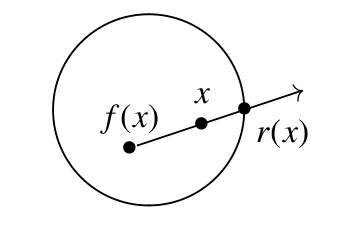
\includegraphics[height=3cm]{img/brouwer-retraction}
      \end{center}

      Define \(r(x)\) to be the point of intersection of this ray. Prove that
      \(r(x)\) is a retraction of \(D^2\) to \(S^1 \subset D^2\). You may take
      for granted that \(r\) is continuous (this follows from continuity of
      \(f\)).

    \item We have retraction \(D^2 \xrightarrow{r} S^1\) and we may extend this
      from the left via the inclusion map
      \[S^1 \xrightarrow{i} D^2 \xrightarrow{r} S^1.\]
      What is the composition \(ri\)?

    \item Use the functoriality of \(\pi_1\) to derive a contradiction in the
      following diagram
      \begin{equation}\label{eq:brouwer-functoriality-diagram}
        \xymatrix{
          S^1 \ar[rr]^i\ar[dd]_{\pi_1} && D^2 \ar[rr]^r\ar[dd]_{\pi_1} && S^1\ar[dd]_{\pi_1}\\
          & &&&\\
          \pi_1(S^1)\ar[rr]^{\pi_1(i)} && \pi_1(D^2)\ar[rr]^{\pi_1(r)} && \pi_1(S^1)
        }\qed{}
      \end{equation}
  \end{enumerate}
  \begin{Solution}
    \begin{enumerate}[(i)]
      \item Let \(x \in S_1 = \partial D^2\) be point on the boundary circle of
        disk \(D^2\). Then the ray from \(f(x)\) to \(x\) intersects \(S^1\) at
        \(x\) and \(r\) restricts to the identity on \(S_1\); that is,

        \[r|_{S_1} = \id_{S_1}.\]

        Choosing function \(i : S^1 \to D^2\) to be the inclusion map of the
        boundary it is easy to see that \(ri : S^1 \to S^1, x \mapsto x\). Now,
        using both the fact that inclusions are continuous and the assumption
        that \(r\) is continuous, we have shown that \(r\) splits arrow \(i\)
        and thus \(r\) is a retraction of \(D^2\) onto \(S^1\).

      \item As noted in (i), \(ri = \id_{S1}\)
      \item By the diagram in~\ref{eq:brouwer-functoriality-diagram} we have
        \(\pi_1(r)\circ \pi_1(i) = \pi_1(ri) = \pi_1(\id_{S^1}) = \id_{\pi_1(S^1)}\).
        But \(\pi_1(S^1) = \Z\) while \(\pi_1(D^2) = 0\) and thus \(\pi_1(i)\)
        is the trivial homomorphism. In particular, \(\pi_1(r)\circ \pi_1(i)\)
        is also trivial and cannot be the identity on \(\Z\).\qed{}
    \end{enumerate}
  \end{Solution}

\end{problem}


\end{document}
